\documentclass[11pt]{article}
\usepackage{amssymb}
\usepackage{amsthm}
\usepackage[fleqn]{amsmath}
\usepackage{listings}
\usepackage{color}
\usepackage{graphicx}
\usepackage{subcaption}
\usepackage{fancyvrb}
\usepackage[colorlinks = true,
            linkcolor = blue,
            urlcolor  = blue,
            citecolor = blue,
            anchorcolor = blue]{hyperref}

\newcommand{\bs}[1]{\boldsymbol{#1}}

\title{A Matlab implementation of L-BFGS-B}
\author{Brian Granzow}
\date{}

\begin{document}

\maketitle

\section{Introduction and motivation}
In this report, we discuss a MATLAB implementation of
the L-BFGS-B \cite{lbfgsb} algorithm for solving
bound-constrained optimization problems of the form:
%
\begin{equation}
\begin{aligned}
& \underset{x}{\text{minimize}}
& & f(x) \\
& \text{subject to}
& & l \leq x \leq u,
\end{aligned}
\end{equation}
%
where $f: \mathbb{R}^n \to \mathbb{R}$ and $x,l,u \in \mathbb{R}^n$.
The L-BFGS-B algorithm is a quasi-Newton gradient-based
optimization algorithm that utilizes limited memory
BFGS approximations to the Hessian matrix,
$\frac{\partial^2 f}{\partial x_i \partial x_j}$, making
it well-suited for optimization problems with a large
number of design variables $n$.

The \href{http://users.iems.northwestern.edu/~nocedal/lbfgsb.html}
{original L-BFGS-B implementation}  \cite{lbfgsb3}
and subsequent releases were implemented in Fortran.
Since its original release,
\href{https://github.com/stephenbeckr/L-BFGS-B-C}{C/C++}
\cite{C},
\href{https://github.com/pcarbo/lbfgsb-matlab}{Matlab}
\cite{Matlab},
\href{https://github.com/mkobos/lbfgsb_wrapper}{Java}
\cite{Java},
and \href{https://github.com/yuhonglin/Lbfgsb.jl}{Julia}
\cite{Julia}
wrappers for the L-BFGS-B Fortan library have been released.
Up to this point, however, an open-source pure Matlab
implementation of the algorithm has been difficult to
come by. This is potentially due to performance reasons,
as the L-BFGS-B algorithm concerns itself mainly with large
scale optimization problems, for which compiled low-level
languages will almost certainly outperform Matlab.

Nevertheless, the aim of this report is to discuss a
recently developed Matlab implementation of the algorithm
that provides Matlab users a convenient way to solve
box-constrained optimization problems with L-BFGS-B using
only a single file Matlab implementation \emph{LBFGS.m},
removing the additional step of installing a third-party
library. This implementation is readily available for use at:
\begin{itemize}
\item \url{https://github.com/bgranzow/L-BFGS-B}{}
\end{itemize}

The remainder of this report is structured as follows.
We begin by presenting a high-level overview of the
L-BFGS-B algorithm, while making appropriate observations
about its Matlab implementation. Then we discuss several
basic regression tests that have been implemented to
ensure the L-BFGS-B Matlab implementation solves
bound-constrained optimization problems appropriately.

\section{The L-BFGS-B algorithm}

From a high-level the L-BFGS-B algorithm iterates over
quasi-Newton steps. For a given iteration $k$,
the objective function is approximated by a quadratic model
at a point $x_k$ as:
%
\begin{equation}
m_k(x) = f_k + g^T_k(x-x_k) + \frac12 (x-x_k)^T B_k (x-x_k),
\label{eq:quadratic}
\end{equation}
%
where $f_k$ represents the objective function $f$ evaluated
at $x_k$, $g_k$ denotes the objective gradient evaluated at
$x_k$, and $B_k$ represents a limited memory BFGS approximation
to the Hessian evaluated at $x_k$. Using this quadratic model,
the L-BFGS-B algorithm can be outlined using the following steps:
%
\begin{enumerate}
\item Check if the inf-norm of the gradient $g_k$ projected onto
the feasible design space is less than a user-specified tolerance.
If it is, then return successfully.
\item Find the Cauchy point $x^c$, that minimizes $m_k$ in
the  steepest descent direction $-g_k$ projected onto the
feasible design space. Once found, the Cauchy point $x^c$
is used to identify active design variables $A(x)$ (those that
are identified as fixed at either an upper or lower bound)
and free variables $F(x)$ (those that are identified as inside the
feasible design space). Conceptually, this is like the algorithm
`peeking ahead' an iteration to determine which variables will
likely be active or inactive.
\item The quadratic model $m_k$ is then minimized for the set
of free variables $F(x)$ in an unconstrained manner, and then
backtracked into the feasible design space to obtain
$\bar{x}_k$.
\item The new search direction is computed as $d_k = \bar{x}_k - x_k$
and a line-search method is used to find a step length $\alpha_k$
that satisfies the strong-Wolfe conditions to compute the new
design variables $x_{k+1}$.
\item The L-BFGS Hessian approximation $B_{k+1}$ is computed based
on the new step $x_{k+1}$ and a new iteration is started.
\end{enumerate}
%
These steps are now discussed from a high-level, with references
to their implementation.

\subsection{Convergence criteria}

Convergence is satisfied if the following criterion holds:
%
\begin{equation}
\| P(x_k - g_k,l,u) - x_k \|_{\infty} < \text{tol},
\end{equation}
%
where tol is a user-specified tolerance and
%
\begin{equation}
P(x,l,u) := 
\begin{aligned}
\begin{cases}
l_i \quad & \text{if} \; x_i < l_i \\
u_i \quad & \text{if} \; x_i > u_i \\
x_i \quad & \text{otherwise}.
\end{cases}
\end{aligned}
\label{eq:projection}
\end{equation}
Note that $P(x_k - g_k,l,u) - x_k$ denotes
the gradient projected onto the feasible design space.
This convergence criteria is computed in the
function
\href{https://github.com/bgranzow/L-BFGS-B/blob/master/LBFGSB.m#L201}
{get\_optimality} in \emph{LBFGS.m}.

\subsection{Computation of the Cauchy point}

For simplicity, we will denote the Hessian
approximation $B_k$, the objective gradient
$g_k$, and the design vector $x_k$ at the $k^{th}$
iteration as $B$, $g$, and $x$, respectively.
The Cauchy point $x^c$ is parameterized
as $x^c = x(t^*)$, where $t^*$ is the first
local minimizer along the piece-wise linear
path $P(t) = P(x-tg,l,u)$, where $P$ was previously
defined in equation \eqref{eq:projection}.
Each coordinate of the piece-wise linear path
$x_i(t)$ is defined as $x_i - t g_i \quad t_i \in [0, t_i]$,
where the breakpoint $t_i$ is given as:
%
\begin{equation}
t_i =
\begin{aligned}
\begin{cases}
(x_i - u_i) / g_i \quad & \text{if} \; g_i < 0, \\
(x_i - l_i) / g_i \quad & \text{if} \; g_i > 0, \\
\infty \quad & \text{otherwise}.
\end{cases}
\end{aligned}
\end{equation}
%
The breakpoints $t_i$ are sorted into an ordered set
$\{t^j : t^{j-1} < t^j, j=1,2,\dots,n \}$
and each interval $[t^{j-1},t^j]$ is subsequently
analyzed until a local minimizer $t^*$ is found.
The details of this minimization process can
be found in Algorithm CP of \cite{lbfgsb}, and
are implemented in the routine
\href{https://github.com/bgranzow/L-BFGS-B/blob/master/LBFGSB.m#L261}
{get\_cauchy\_point} in \emph{LBFGS.m}.

\subsection{Subspace minimization}

Once the Cauchy point $x^c$ has been computed, the
quadratic model $m_k$ is minimized for the free
variables of $x^c$, those whose values are not equal to upper
or lower bound values, in an unconstrained manner to
obtain a solution vector $d^u$. This is done by directly
inverting the L-BFGS-B Hessian approximation $B_k$ using
the Sherman-Morrison-Woodbury formula. Once the unconstrained minimizer
is found, it is backtracked towards the feasible region with a
positive scaling parameter $\alpha^*$ to provide a backtracked solution
vector $d_k = \alpha^* d^u$. This provides enough information to compute
$\bar{x}_k$, the minimization to the subspace problem with
the bounds imposed on the design variables.
The details of the subspace minimization
are given in Section 5.1 of \cite{lbfgsb} and the method
is implemented
in \emph{LBFGS.m} in the routine
\href{https://github.com/bgranzow/L-BFGS-B/blob/master/LBFGSB.m#L358}
{subspace\_min}.

\subsection{Strong-Wolfe line search}

The new search direction is then given as $d_k = \bar{x}_k - x_k$.
A line search algorithm is performed in this direction to find
a step length $\alpha_k$ that satisfies the strong-Wolfe
conditions given by the sufficient decrease condition:
%
\begin{equation}
f(x_{k+1}) \leq f(x_k) + c_1 \alpha_k g_k^T d_k,
\end{equation}
%
and the curvature condition:
%
\begin{equation}
| g^T_{k+1}  d_k | \leq c_2 | g^T_k d_k |,
\end{equation}
%
where $c_1$ and $c_2$ are chosen to be $10^{-4}$ and
$0.9$, respectively.
The algorithm to compute this line search is given
by Algorithms 3.5 and 3.6 of the reference
\cite{optimization}, and is implemented in
\emph{LBFGS.m} in the routine
\href{https://github.com/bgranzow/L-BFGS-B/blob/master/LBFGSB.m#L427}
{strong\_wolfe}.

\subsection{L-BFGS updates}

Limited memory BFGS Hessian approximations store $m$ iteration
pairs $Y_k = [y_{k-m}, y_{k-m+1}, \dots, y_{k-1}]$ and
$S_k = [s_{k-m}, s_{k-m+1}, \dots, s_{k-1}]$ where
$y_k = g_k - g_{k-1}$ and $s_k = x_k - x_{k-1}$. Here the
Hessian approximation $B_k$ can be written as:
%
\begin{equation}
B_k = \theta I - W_k M^{-1}_k W^T_k.
\end{equation}
%
The expressions for the matrices $W_k$ and $M_k$ are
outlined in Section 3 of reference \cite{lbfgsb}. The updates
to the L-BFGS data structures occur inside the quasi-Newton
iterations in \emph{LBFGS.m} starting on
\href{https://github.com/bgranzow/L-BFGS-B/blob/master/LBFGSB.m#L66}{line 66}.

\section{Results}

\subsection{Convex quadratic functions}

The \href{https://github.com/bgranzow/L-BFGS-B/blob/master/test_LBFGSB.m}
{LBFGS.m} implementation is bundled with a series of basic
\href{https://github.com/bgranzow/L-BFGS-B/blob/master/test_LBFGSB.m}
{regression tests} that ensure the algorithm performs as
expected for the two simple objective functions:
%
\begin{equation}
f_1(x) = x^T x,
\end{equation}
and
\begin{equation}
f_2(x) = - x^T x.
\end{equation}
%
with $n = 100$ design variables, $m=10$ stored iteration
pairs for the L-BFGS data structures, and a convergence
tolerance of $10^{-5}$. Using these two objective
functions, six regression tests are defined.

The
\href{https://github.com/bgranzow/L-BFGS-B/blob/master/test_LBFGSB.m#L10}
{first regression test} is defined as the problem
%
\begin{equation}
\begin{aligned}
& \underset{x}{\text{minimize}}
& & f_1(x) \\
& \text{subject to}
& & -10 \leq x \leq 10,
\end{aligned}
\end{equation}
%
with the initial starting guess $x_i = 5 \; \forall i$.
The solution behaves essentially as an unconstrained
optimization problem and converges in a single quasi-Newton
iteration to the correct solution
$x_i = 0 \; \forall i$.

The
\href{https://github.com/bgranzow/L-BFGS-B/blob/master/test_LBFGSB.m#L24}
{second regression test} is identical to the first,
with the exception that the lower bound is set to $l = 1$
rather than $-10$. Again this regression test converges in a single
quasi-Newton iteration to the correct solution
$x_i = 1 \; \forall i$.

The
\href{https://github.com/bgranzow/L-BFGS-B/blob/master/test_LBFGSB.m#L38}
{third regression test} is identical to the first,
with the exception that the initial guess is defined outside
of the box-constraints, such that $x_i = -20 \; \forall i$.
This test converges in two quasi-Newton iterations to the
correct solution $x_i = 0 \; \forall i$.

The
\href{https://github.com/bgranzow/L-BFGS-B/blob/master/test_LBFGSB.m#L52}
{fourth regression test} is defined as
%
\begin{equation}
\begin{aligned}
& \underset{x}{\text{minimize}}
& & f_1(x) \\
& \text{subject to}
& & 1 \leq x \leq 10,
\end{aligned}
\end{equation}
%
with the initial guess defined as a random
vector whose components satisfy $9 \leq x_i \leq 10 \; \forall i$.
This test converges to the correct solution
$x_i = 1 \; \forall i$ in one quasi-Newton iteration.

To verify upper bounds can be properly satisfied, the
\href{https://github.com/bgranzow/L-BFGS-B/blob/master/test_LBFGSB.m#L66}
{fifth regression test} is defined as:
%
\begin{equation}
\begin{aligned}
& \underset{x}{\text{minimize}}
& & f_2(x) \\
& \text{subject to}
& & 0 \leq x \leq 10,
\end{aligned}
\end{equation}
%
where the initial design vector is chosen as
$x_i = 5 \; \forall i$. This test converges
correctly to the solution $x_i = 10 \; \forall i$
in one quasi-Newton iteration.

Finally, the
\href{https://github.com/bgranzow/L-BFGS-B/blob/master/test_LBFGSB.m#L80}
{sixth test} is defined such that
a non-uniform lower bound constraint is set,
where the optimization problem is defined as:
\begin{equation}
\begin{aligned}
& \underset{x}{\text{minimize}}
& & f_1(x) \\
& \text{subject to}
& & \sin(\pi \frac{1-i}{n}) \leq x_i \leq 10  \quad \forall i
\end{aligned}
\end{equation}
%
which correctly converges to the solution
$x_i = \sin(\pi \frac{1-i}{n}) \; \forall i$ in
one quasi-Newton iteration.

\subsection{A bounded Rosenbrock example}

As a more extensive test of the L-BFGS-B implementation,
a bounded Rosenbrock
\href{https://github.com/bgranzow/L-BFGS-B/blob/master/test_rosenbrock.m}
{example}, is included in the source distribution.
We consider the Rosenbrock function defined as:
%
\begin{equation}
f_3(x) = 100(x_2-x_1^2)^2 + (1-x_1)^2,
\end{equation}
%
where $x \in \mathbb{R}^2$.
We first use the L-BFGS-B algorithm to solve the
unconstrained minimization problem
%
\begin{equation}
\begin{aligned}
& \underset{x}{\text{minimize}}
& & f_3(x) \\
& \text{subject to}
& & -\infty < x < \infty  \quad
\end{aligned}
\end{equation}
%
with the initial guess $(x_1,x_2) = (-1.2, 1)$, using
$m=10$ stored L-BFGS iteration pairs and a maximum
number of quasi-Newton iterations of $100$.
The search path for the unconstrained problem is
shown in Figure \ref{fig:rosenbrock_unconstrained}.
%
\begin{figure}[hbt!]
\centering
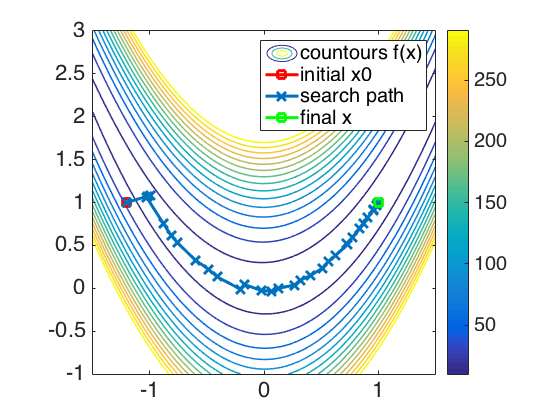
\includegraphics[width=0.75\textwidth]{rosenbrock_unbounded}
\caption{Search history for the unconstrained Rosenbrock example}
\label{fig:rosenbrock_unconstrained}
\end{figure}
%
Without active bound variables, the L-BFGS-B method essentially
reduces to the standard L-BFGS method. This result gives us
confidence that the L-BFGS data structures and updates
are performed correctly in the \emph{LBFGS.m} implementation.
The convergence history for the unconstrained Rosenbrock
problem is shown in Figure \ref{fig:ros_unc_conv}.
%
\begin{figure}[hbt!]
\scriptsize
\centering
\begin{BVerbatim}
 iter        f(x)          optimality
-------------------------------------
  0      24.20000000     215.60000000
  1       5.10111266      38.33803031
  2       4.15378843       6.65579078
  3       4.11721504       1.40757360
  4       4.10921995       1.42455138
  5       4.10922456       1.42457526
  6       3.58186385      11.18575152
  7       3.45470246      17.47839459
  8       3.28544194      16.76380586
  9       2.65947615      10.87782125
 10       2.22970801       5.83940028
 11       2.09539857       8.36664503
 12       1.75072527      11.07438171
 13       1.39706792       2.79021511
 14       1.11088550       4.82357799
 15       1.03878169       8.04442772
 16       0.79586966       3.26617858
 17       0.64945895       6.65883593
 18       0.46730756       1.11095742
 19       0.38120958       3.61380605
 20       0.30770768       5.10591921
 21       0.19454187       0.57434669
 22       0.15033422       2.04613244
 23       0.12796165       6.48492562
 24       0.07920583       0.77105145
 25       0.05289519       0.49482493
 26       0.03442939       2.68276032
 27       0.01970635       1.93274402
 28       0.00863828       0.32795662
 29       0.00470913       1.91555193
 30       0.00202819       0.48371906
 31       0.00035537       0.22332188
 32       0.00004326       0.18103267
 33       0.00000213       0.03578927
 34       0.00000012       0.00998035
 35       0.00000000       0.00006825
 36       0.00000000       0.00000511
\end{BVerbatim}
\caption{Convergence history for the unbounded Rosenbrock example}
\label{fig:ros_unc_conv}
\end{figure}

As a second example, the Rosenbrock problem is modified
to include a box constraint, such that the new problem
definition is given as:
\begin{equation}
\begin{aligned}
& \underset{x}{\text{minimize}}
& & f_3(x) \\
& \text{subject to}
& & -0.5 \leq x_1 \leq 0.5, \\
& & & -0.5 \leq x_2 \leq 0.5,
\end{aligned}
\end{equation}
%
where the initial guess is again given as
$(x_1, x_2) = (-1.2, 1.0)$.
The search path produced by the \emph{LBFGS.m} implementation
is shown in Figure \ref{fig:rosenbrock_constrained}. Notice
that the initial design is outside of the box constraints.
The \emph{LBFGS.m} projects the initial design guess onto
the feasible design space for the first iteration, and then
proceeds as normal for subsequent iterations. Notice
that once the design vector enters the `banana valley',
it takes approximately the same path towards the global
minimum that the unbounded Rosenbrock example takes.
However, it finds a bounded minimum at the design location
$x = (0.5,0.25)$. This result was corroborated by
comparison to a result obtained via Matlab's robust optimization
solver \emph{fmincon}. The convergence history for the
bounded Rosenbrock example is shown in Figure \ref{fig:ros_con_conv}.
%
\begin{figure}[hbt]
\centering
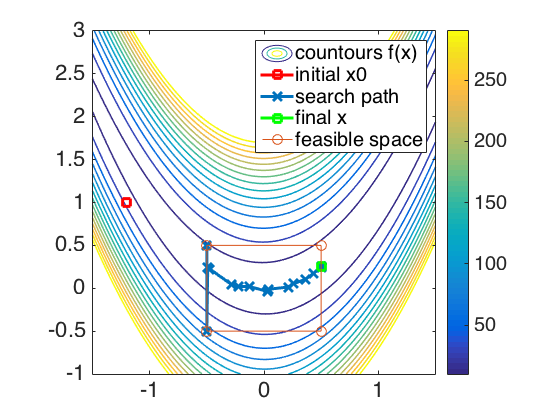
\includegraphics[width=0.75\textwidth]{rosenbrock_bounded}
\caption{Search history for constrained Rosenbrock example}
\label{fig:rosenbrock_constrained}
\end{figure}
%
\begin{figure}[hbt!]
\scriptsize
\centering
\begin{BVerbatim}
 iter        f(x)          optimality
-------------------------------------
  0       8.50000000       1.00000000
  1      58.50000000       1.00000000
  2       2.22755657       0.99250000
  3       2.17219686       0.97383645
  4       1.78942574       0.78413677
  5       1.58869314       0.72538530
  6       1.26415453       0.62376555
  7       1.08833255       0.53790684
  8       0.93554003       0.51145792
  9       0.71623471       0.71067169
 10       0.56619271       0.44590189
 11       0.47950989       0.85958247
 12       0.34314773       0.93149460
 13       0.25780652       0.76709009
 14       0.25011825       0.21748547
 15       0.25000000       0.00000000
\end{BVerbatim}
\caption{Convergence history for the unbounded Rosenbrock example}
\label{fig:ros_con_conv}
\end{figure}

\section{Conclusions}

We have implemented a pure Matlab implementation of
the L-BFGS-B algorithm for box-constrained gradient-based
optimization. We have provided a high-level overview
of the fundamental steps of the algorithm and provided
references to the corresponding implementation
locations of these steps in the \emph{LBFGS.m} code.
The implementation has been verified for a series of
simple tests. Further work includes verifying the
implementation for a wider variety of optimization
problems.

\begin{thebibliography}{99}

\bibitem{lbfgsb}
Byrd, R. H., Lu, P., Nocedal, J., \& Zhu, C. (1995).
\emph{A limited memory algorithm for bound constrained optimization}.
SIAM Journal on Scientific Computing, 16(5), 1190-1208.

\bibitem{optimization}
Nocedal, J. and Wright, S.
\emph{Numerical optimization}. Springer Science \& Business Media, 2006.

\bibitem{lbfgsb3}
Byrd, R. H., Lu, P., Nocedal, J., \& Zhu, C.
\emph{L-BFGS-B}.
\url{http://users.iems.northwestern.edu/~nocedal/lbfgsb.html}.
Accessed: 2016-12-13.

\bibitem{C}
Becker, S.
\emph{L-BFGS-B-C}
\url{https://github.com/stephenbeckr/L-BFGS-B-C}.
Accessed: 2016-12-13.

\bibitem{Matlab}
Carbonetto, P.
\emph{lbfgsb-matlab}.
\url{https://github.com/pcarbo/lbfgsb-matlab}.
Accessed: 2016-12-13.

\bibitem{Java}
Kobos, M.
\emph{lbfgsb\_wrapper}
\url{https://github.com/mkobos/lbfgsb_wrapper}.
Accessed: 2016-12-13.

\bibitem{Julia}
Yu, H.
\emph{Lbfgsb.jl}.
\url{https://github.com/yuhonglin/Lbfgsb.jl}.
Accessed: 2016-12-13.

\bibitem{LBFGS}
Byrd, Richard H., Jorge Nocedal, and Robert B. Schnabel.
\emph{Representations of quasi-Newton matrices and their
use in limited memory methods}.
Mathematical Programming 63.1-3 (1994): 129-156.

\end{thebibliography}

\newpage

\end{document}
